\documentclass[crop,tikz,convert={outext=.svg,command=\unexpanded{pdf2svg \infile\space\outfile}},multi=false]{standalone}
\usepackage[utf8]{inputenc}
\usepackage[dvipsnames]{xcolor} 
\usepackage{fancyhdr}
\usepackage{ucs} 
\usepackage{todonotes}
\usepackage{graphicx}
\usetikzlibrary{shapes}
\usetikzlibrary{shapes,arrows}
\usetikzlibrary{decorations.pathmorphing, decorations.text}
\usepackage{makeidx}
\usepackage{booktabs}
\usepackage{pdfpages}
\usepackage{ngerman}
%\usepackage{fontspec}
%\setmainfont{Arial}
\tikzstyle{every picture}+=[font=\sffamily]


\begin{document}
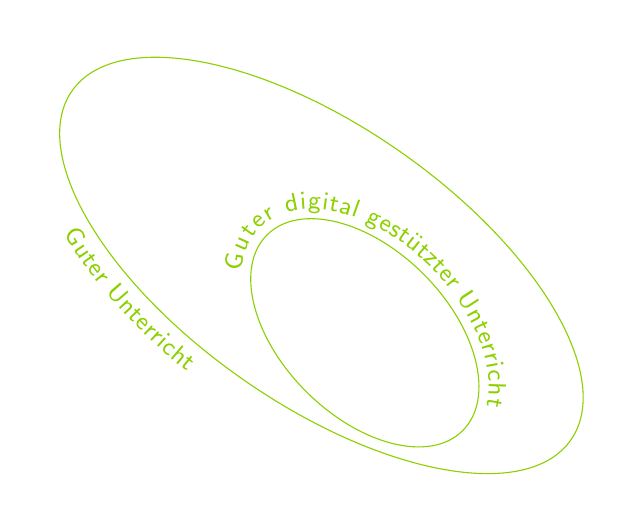
\begin{tikzpicture}
  
  
\definecolor{todesgruen}{HTML}{8cd000}  
%%     
\draw[rotate=+55, 
      color = todesgruen,
      postaction={decorate,
      decoration={raise=-1em, 
      text along path, pre length=6.3cm,
      text={|\sffamily \small \color{todesgruen}|Guter Unterricht},
    },
  }] (0,0) arc (0:360:50pt and 110pt);  
  

  
\draw[rotate=-135, 
      color = todesgruen,
 postaction={decorate,
    decoration={raise=.35em, 
    text along path, pre length=1.7cm,
      text={|\sffamily \small \color{todesgruen}|Guter digital gest{ü}tzter Unterricht},
    },
  }] (3,1.3) arc (360:0:30pt and 50pt);
  



 
\end{tikzpicture}
\end{document}
